%% electric-eye: real-time image enhancement and low-latency video transport for
%% remotely operated underwater vehicles. Material and methods.
%%
%% In the Elsevier CAS single-column template (cas-sc.cls, cas-common.sty,
%% cas-model2-names.bst), as the ayzek manuscript.
%%
%%   make            paper.pdf
%%
%% Every figure but one is drawn in TikZ here; figures/fig3_autovis.png is
%% rendered from the frames of the software's own test (tests/test_auto_vis.c).
\documentclass[a4paper,fleqn]{cas-sc}

\usepackage[authoryear]{natbib}
\usepackage{graphicx}
\usepackage{amsmath}
\usepackage{booktabs}
\usepackage{makecell}
\usepackage{array}
\usepackage{setspace}
\usepackage{lineno}
\usepackage{tikz}
\usetikzlibrary{positioning,arrows.meta,fit,backgrounds,calc}
% The template's \cortext ends up printing its "[COR: Number]" trace on the
% first page in this build; send the trace to the log only.
\ExplSyntaxOn
\cs_set_protected:Npn \msg_term:n #1 { \iow_log:n {#1} }
\ExplSyntaxOff
\makeatletter
\AddToHook{shipout/before}{\immediate\write\@auxout{\string\csxdef{lastpage}{\thepage}}}
\makeatother
\linenumbers

\newcommand{\eeye}{\texttt{eeye}}
\newcommand{\hellion}{\texttt{hellion}}
\newcommand{\tablenote}[1]{\par\vspace{4pt}%
  \begin{minipage}{\linewidth}\footnotesize\textit{Note.} #1
\end{minipage}}
\newcolumntype{L}[1]{>{\raggedright\arraybackslash}p{#1}}

% Figure styles: processes, buffers and data paths.
\tikzset{
  proc/.style={draw, rounded corners=2pt, fill=gray!8, align=center,
    font=\footnotesize, minimum height=7mm, inner sep=3pt},
  buf/.style={draw, fill=white, align=center, font=\footnotesize,
    minimum height=6mm, inner sep=3pt},
  ext/.style={draw, dashed, align=center, font=\footnotesize, minimum height=7mm,
    inner sep=3pt},
  box/.style={draw, rounded corners=4pt, inner sep=6pt},
  flow/.style={-{Stealth[length=2mm]}, semithick},
  net/.style={-{Stealth[length=2mm]}, very thick},
  lab/.style={font=\scriptsize, align=center},
}

\begin{document}
\let\WriteBookmarks\relax
\def\floatpagepagefraction{1}
\def\textpagefraction{.001}
\shorttitle{Real-time enhancement and low-latency transport for underwater vehicles}
\shortauthors{H.O. Bolat and H. Ersoy}

\title [mode = title]{electric-eye: Real-Time Image Enhancement and Low-Latency Video
Transport for Remotely Operated Underwater Vehicles}

\author[1]{H. O\u{g}uz Bolat}[orcid=0009-0000-8522-7746]
\cormark[1]
\ead{oguz.bolat@std.yildiz.edu.tr}
\credit{Conceptualization, Methodology, Software, Validation, Investigation,
Writing -- original draft}

\author[2]{Hakan Ersoy}
\credit{Writing -- review and editing}

\address[1]{Department of Geomatics Engineering, Y\i{}ld\i{}z Technical University,
Davutpa\c{s}a Campus, 34220 Esenler, \.Istanbul, T\"urkiye}
\address[2]{Department of Electronics and Communication Engineering, Y\i{}ld\i{}z
Technical University, Davutpa\c{s}a Campus, 34220 Esenler, \.Istanbul, T\"urkiye}

\cortext[1]{Corresponding author}

\begin{abstract}
  The pilot of a remotely operated vehicle steers by a video picture that turbid water
  degrades and that a tether carries with delay, and image processing inserted between
  the camera and the pilot must add as little delay as it can. We describe
  electric-eye, two C99 programs for GNU/Linux that sit between an ROV's camera and its
  pilot. \eeye{} applies a chain of image operators (point operations fused into
  look-up tables, blur, Sobel, Laplacian-of-Gaussian and Canny edges) and an optional
  continuous visibility correction (cast removal, contrast stretch and contrast-limited
  adaptive histogram equalization, smoothed over time), and publishes frames on a
  shared-memory frame bus that never waits for its readers. \hellion{} carries the
  picture across the tether as H.264 over RTP, relays the vehicle's packets to
  QGroundControl unchanged, records them, measures the link, serves a browser control
  page, and finds its counterpart on the network by itself. Either program can run on
  either side of the tether. Two changes on the receiving side, an end-of-frame
  delimiter inserted by the relay and slice-threaded decoder output, reduced the
  transport latency from bus to bus over loopback from 70.4 to 3.8~ms at
  640$\times$480 and from 74.8 to 8.3~ms at 1280$\times$720. The visibility correction
  costs 0.55~ms per 1280$\times$720 frame on four desktop threads. Optimizations that
  should not change the output were checked byte for byte against the previous code on
  x86-64 and, under emulation, on ARMv7 and AArch64. The software has not yet been run
  on a vehicle; code and release binaries are open.
\end{abstract}

\begin{keywords}
  Remotely operated vehicle \sep Underwater imaging \sep Image enhancement \sep
  Low-latency video \sep RTP \sep Embedded Linux
\end{keywords}

\maketitle

\doublespacing

\section{Material and methods}\label{sec:methods}

\subsection{System overview}\label{sec:overview}

The pipeline processes the video of a remotely operated vehicle (ROV) between its
camera and the pilot. It was built for a BlueROV2 \citep{bluerov2}, whose onboard
Raspberry Pi runs BlueOS and the ArduSub autopilot \citep{ardusub} and is joined to a
topside computer by an Ethernet tether, and it runs on any GNU/Linux machine. It
consists of two programs (Figure~\ref{fig:overview}). \eeye{}, the vision layer, takes
frames from a camera or from the tether, applies a configurable chain of image
operators and an optional continuous visibility correction, and publishes the result
(\emph{pilot}) and the untouched camera frame (\emph{raw}) on a shared-memory
\emph{frame bus} for any other program on the machine; it has no network code.
\hellion{} does everything that crosses the tether: it encodes the video as H.264
\citep{itu_h264} over RTP \citep{rfc3550,rfc6184}, receives it topside, relays it to
QGroundControl \citep{qgroundcontrol}, records it, serves a browser control page, and
carries \eeye{}'s settings from the page to wherever \eeye{} runs. The two programs
communicate only through the frame bus and \eeye{}'s configuration file, so either can
be restarted without the other.

\eeye{} runs on one side of the tether, chosen at installation (the \emph{placement};
Figure~\ref{fig:overview}). In placement~B it runs on the vehicle next to the camera,
the vehicle sends the processed picture, and the topside relays the received packets to
QGroundControl unchanged, so the picture is encoded once. In placement~A the vehicle
sends its camera, \eeye{} runs topside on the decoded stream, and the processed picture
is encoded a second time for QGroundControl; this moves the image processing off the
vehicle's processor. Autonomy code is expected to run next to \eeye{} and read
\emph{raw} from the bus, so that its input is the camera's frame and carries the
camera's timestamps.

\begin{figure}[pos=htbp]
  \centering
  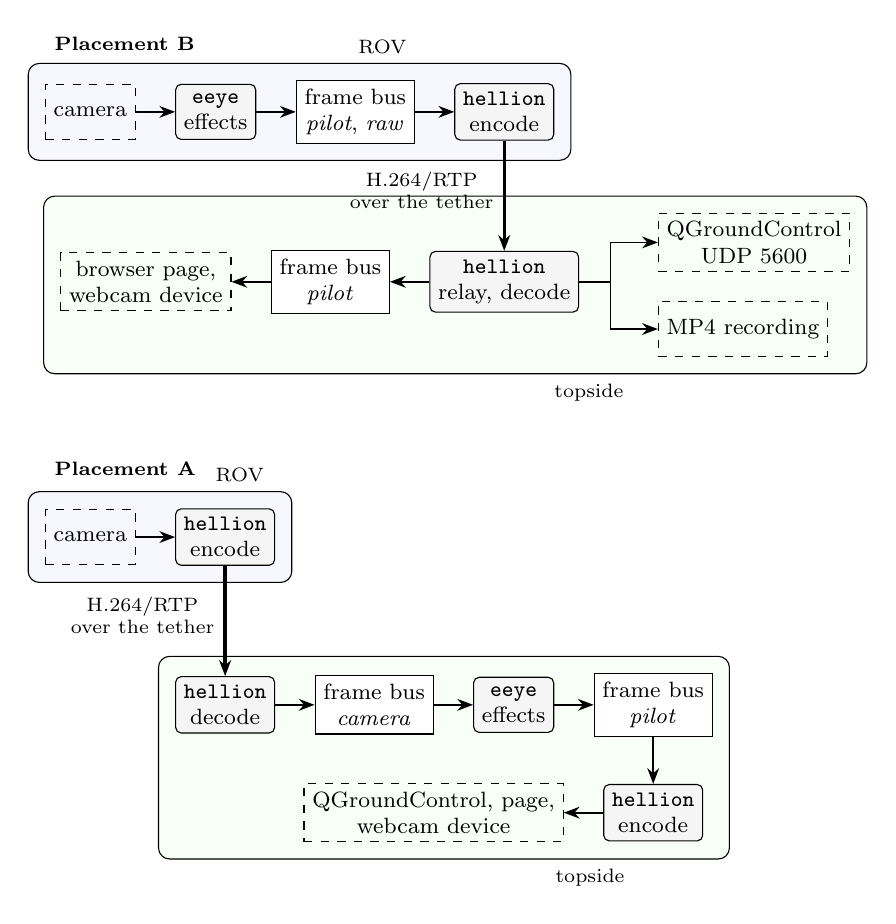
\begin{tikzpicture}[node distance=4mm and 5mm]
    % Placement B
    \node[lab, anchor=west] (bt) at (0,0) {\textbf{Placement B}};
    \node[ext, below=3mm of bt.south west, anchor=north west] (cam) {camera};
    \node[proc, right=of cam] (ee) {\eeye{}\\effects};
    \node[buf, right=of ee] (bus) {frame bus\\\emph{pilot}, \emph{raw}};
    \node[proc, right=of bus] (hr) {\hellion{}\\encode};
    \node[proc, below=14mm of hr] (ht) {\hellion{}\\relay, decode};
    \node[ext, right=10mm of ht, yshift=5mm] (qgc) {QGroundControl\\UDP 5600};
    \node[ext, right=10mm of ht, yshift=-6mm] (rec) {MP4 recording};
    \node[buf, left=of ht] (tbus) {frame bus\\\emph{pilot}};
    \node[ext, left=of tbus] (page) {browser page,\\webcam device};
    \draw[flow] (cam) -- (ee);
    \draw[flow] (ee) -- (bus);
    \draw[flow] (bus) -- (hr);
    \draw[net] (hr) -- node[lab, left, pos=0.45] {H.264/RTP\\over the tether} (ht);
    \draw[flow] (ht.east) -- ++(4mm,0) |- (qgc.west);
    \draw[flow] (ht.east) -- ++(4mm,0) |- (rec.west);
    \draw[flow] (ht) -- (tbus);
    \draw[flow] (tbus) -- (page);
    \begin{scope}[on background layer]
      \node[box, fill=blue!3, fit=(cam)(ee)(bus)(hr), label={[lab]above right:ROV}] {};
      \node[box, fill=green!3, fit=(page)(tbus)(ht)(qgc)(rec),
            label={[lab]below right:topside}] {};
    \end{scope}
    % Placement A
    \node[lab, anchor=west] (at) at (0,-5.4) {\textbf{Placement A}};
    \node[ext, below=3mm of at.south west, anchor=north west] (camA) {camera};
    \node[proc, right=of camA] (hrA) {\hellion{}\\encode};
    \node[proc, below=14mm of hrA] (htA) {\hellion{}\\decode};
    \node[buf, right=of htA] (busA) {frame bus\\\emph{camera}};
    \node[proc, right=of busA] (eeA) {\eeye{}\\effects};
    \node[buf, right=of eeA] (busA2) {frame bus\\\emph{pilot}};
    \node[proc, below=6mm of busA2] (heA) {\hellion{}\\encode};
    \node[ext, left=of heA] (qgcA) {QGroundControl, page,\\webcam device};
    \draw[flow] (camA) -- (hrA);
    \draw[net] (hrA) -- node[lab, left, pos=0.45] {H.264/RTP\\over the tether} (htA);
    \draw[flow] (htA) -- (busA);
    \draw[flow] (busA) -- (eeA);
    \draw[flow] (eeA) -- (busA2);
    \draw[flow] (busA2) -- (heA);
    \draw[flow] (heA) -- (qgcA);
    \begin{scope}[on background layer]
      \node[box, fill=blue!3, fit=(camA)(hrA), label={[lab]above right:ROV}] {};
      \node[box, fill=green!3, fit=(htA)(busA)(eeA)(busA2)(heA)(qgcA),
            label={[lab]below right:topside}] {};
    \end{scope}
  \end{tikzpicture}
  \caption{The two programs and the two placements. In placement B, used on the
    vehicle, \eeye{} processes the camera on the ROV, and QGroundControl receives the
    ROV's packets unchanged. In placement A the ROV sends its camera and the
    processing runs topside, at the cost of a second encode. Programs on one machine
    exchange frames only through the frame bus.}\label{fig:overview}
\end{figure}

\subsection{Image acquisition}\label{sec:capture}

\eeye{} captures from a USB (UVC) camera through V4L2 \citep{v4l2} with memory-mapped
streaming, or from a Raspberry Pi camera module through a \texttt{rpicam-vid}
\citep{rpicamapps} child process; a third source reads a frame bus stream
(placement~A). On V4L2 it takes MJPEG when the camera offers it at the requested size
and packed 4:2:2 (YUYV) otherwise, because at USB~2.0 bandwidth most cameras offer
720p only as MJPEG. When the requested size is not offered, the closest mode is chosen
by aspect ratio first and pixel count second, once at startup, since all frame buffers
are allocated at that size. MJPEG is decoded with libjpeg-turbo \citep{libjpegturbo}
directly into 4:2:2 planes; an optional downscale by 2, 4 or 8 is applied inside the
decoder (by dropping DCT coefficients) or, for YUYV, while the packed samples are
deinterleaved.

Every frame is held as planar I422 at full range (0--255 for luma and chroma, the range
the operators assume; \citealp{itu_bt601}). It carries a frame number and its capture
time on \texttt{CLOCK\_MONOTONIC}: the driver's buffer timestamp when the driver
stamps that clock, otherwise the time of receipt. Each capture takes, after the first
ready buffer, every further buffer the driver has filled, returns the older ones
unread and decodes only the newest; when all buffers fill, the V4L2 driver keeps the
oldest frames and drops new ones, and without this a single slow frame left the
picture permanently several frames behind.

Camera controls (exposure, gain, white balance, brightness, contrast, saturation,
sharpness) are expressed in device-independent units, percentages of the device's
reported range or physical units (exposure in microseconds, white balance in kelvin),
and are mapped onto each camera's own range. A field left out leaves that control
untouched. One control is set by default: the V4L2 control that lets automatic
exposure lengthen the shutter beyond the frame period is turned off, because with it
on the laptop camera used for testing (Section~\ref{sec:verification}) fell from 30 to
17~frames per second in a dim room, and every later stage inherits the rate. In
placement~A the controls travel from the topside to the vehicle's \hellion{}, which
holds the camera, applies them, and keeps them for its next start.

\subsection{Processing threads and buffers}\label{sec:threads}

Inside \eeye{} a producer thread captures, an effects thread runs the operators, and
a consumer thread publishes (Figure~\ref{fig:eeye}). The threads pass frames through
three ring buffers of 32 slots, and frames come from a pool of eight that is allocated
once and never grows, so that the pool size bounds the lag between capture and output
(eight frames, 267~ms at 30~frames per second). Each frame has three planar buffers:
the untouched capture (\emph{raw}), the working image, and a spare that lets two
consecutive neighbourhood operators alternate without copying.

The configuration is a JSON file that a watcher thread reloads within milliseconds of
any change (inotify). A parsed configuration is published by an atomic pointer swap,
and the effects thread takes one snapshot per frame, so that no frame is processed
with two configurations. After every load \eeye{} writes whether it accepted the file;
\hellion{}, which writes the file for the browser page, waits for that verdict and
puts the previous file back when the new one is refused. Once a second the consumer
assembles a health record (capture state, frame count, recording state and the image
statistics of Section~\ref{sec:autovis}); the stats thread writes it, so that file
input/output on the vehicle's SD card cannot stall the thread that publishes the
pilot's picture.

\begin{figure}[pos=htbp]
  \centering
  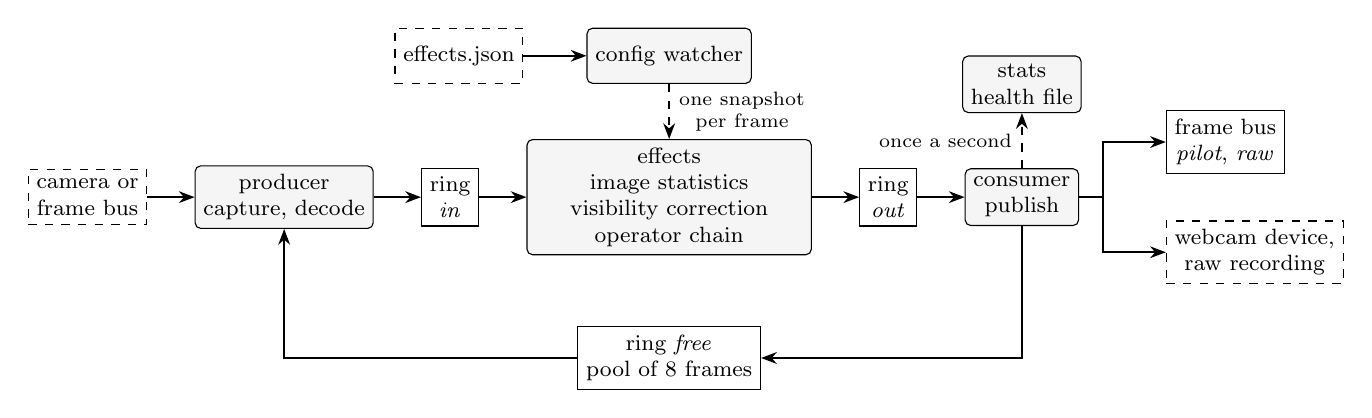
\begin{tikzpicture}[node distance=5mm and 6mm]
    \node[ext] (cam) {camera or\\frame bus};
    \node[proc, right=of cam] (prod) {producer\\capture, decode};
    \node[buf, right=of prod] (rin) {ring\\\emph{in}};
    \node[proc, right=of rin, text width=34mm] (eff) {effects\\image statistics\\visibility correction\\operator chain};
    \node[buf, right=of eff] (rout) {ring\\\emph{out}};
    \node[proc, right=of rout] (cons) {consumer\\publish};
    \node[buf, below=9mm of eff] (rfree) {ring \emph{free}\\pool of 8 frames};
    \node[buf, right=11mm of cons, yshift=7mm] (bus) {frame bus\\\emph{pilot}, \emph{raw}};
    \node[ext, right=11mm of cons, yshift=-7mm] (out) {webcam device,\\raw recording};
    \node[proc, above=7mm of eff] (cfg) {config watcher};
    \node[ext, left=8mm of cfg] (file) {effects.json};
    \node[proc, above=7mm of cons] (stats) {stats\\health file};
    \draw[flow] (cam) -- (prod);
    \draw[flow] (prod) -- (rin);
    \draw[flow] (rin) -- (eff);
    \draw[flow] (eff) -- (rout);
    \draw[flow] (rout) -- (cons);
    \draw[flow] (cons.east) -- ++(3mm,0) |- (bus.west);
    \draw[flow] (cons.east) -- ++(3mm,0) |- (out.west);
    \draw[flow] (cons.south) |- (rfree.east);
    \draw[flow] (rfree.west) -| (prod.south);
    \draw[flow] (file) -- (cfg);
    \draw[flow, dashed] (cfg) -- node[lab, right] {one snapshot\\per frame} (eff);
    \draw[flow, dashed] (cons) -- node[lab, left] {once a second} (stats);
  \end{tikzpicture}
  \caption{Threads and buffers of \eeye{}. Frames circulate from the free ring through
    capture, processing and publication and back; the pool of eight frames bounds the
    output lag. Configuration changes reach the effects thread as whole snapshots.
    The stats thread writes the health file, so that file input/output never runs on
    the consumer.}\label{fig:eeye}
\end{figure}

\subsection{Image operators}\label{sec:operators}

The operator chain holds up to eight stages applied in order; Table~\ref{tab:operators}
lists the operators. Point operators (grayscale, invert, threshold, tint, light)
are composed into one 256-entry lookup table per plane for each run of consecutive
point stages, so that a run costs one pass over the frame whatever its length. The
neighbourhood operators read 3$\times$3 or 5-sample neighbourhoods and replicate the
border samples, because zero padding would produce a false response along the frame
edge.

The Gaussian blur repeats a separable binomial kernel,
\begin{equation}\label{eq:blur}
  g(x) = \left\lfloor \frac{p_{x-2} + 4p_{x-1} + 6p_x + 4p_{x+1} + p_{x+2} + 8}{16}
  \right\rfloor ,
\end{equation}
horizontally and then vertically, $s$ times for strength $s$; repeated passes widen
the effective Gaussian as $\sqrt{s}$. Each thread computes its own band of output rows
in a single sweep, keeping the five horizontally filtered rows it needs in a rolling
window, and successive passes alternate between the destination and a scratch plane,
which needs one synchronization of the thread team per pass where filtering in place
needs two. From $s = 4$ the passes run at half resolution: the plane is reduced by
2$\times$2 averaging, blurred, and expanded by bilinear interpolation with weights
$\tfrac34$ and $\tfrac14$.

Sobel \citep{duda1973} computes the gradients $G_x$ and $G_y$ of the 3$\times$3 Sobel
kernels and outputs $\min(|G_x| + |G_y|, 255)$, set to zero below a threshold.
The Laplacian-of-Gaussian operator \citep{marr1980} blurs with
Eq.~\eqref{eq:blur}, takes the 4-neighbour Laplacian in 16-bit signed arithmetic and
marks a pixel where the response changes sign towards its right or lower neighbour by
at least a threshold; comparing in two directions only keeps contours one pixel wide,
and the slope test rejects noise that merely grazes zero. Canny's detector
\citep{canny1986} is implemented in four stages: at least one blur pass, which keeps
the cost of hysteresis bounded on noisy input; the Sobel gradient, with its direction
quantized to four sectors by integer comparisons ($|G_y| < 0.4|G_x|$ horizontal,
$|G_y| > 2.4|G_x|$ vertical, otherwise diagonal by the signs of $G_x$ and $G_y$);
non-maximum suppression, keeping a pixel when it is not below one neighbour across the
edge and strictly above the other, which thins a symmetric ridge to one pixel; and
hysteresis. Suppression labels each pixel directly in the output, as a seed when its
magnitude reaches the high threshold and as a candidate when it reaches the low one;
each row's seeds are collected as it is labelled; a serial flood fill from the seeds
promotes connected candidates, and a final parallel pass clears the candidates it did
not reach. The flood fill gives the exact connected set, which a parallel sweep would
only approximate.

The edge operators output luma only and set the chroma planes to the neutral value
128. A pass that computes chroma no later stage will read (a blur, tint or contrast
stretch before an edge operator, for example) is skipped; the stages after the last
one that writes chroma are traced back once per configuration. When a chain's output
chroma is known to be neutral, the frame is marked and the frame bus copies only luma
(Section~\ref{sec:bus}).

The neighbourhood operators have NEON implementations, written with intrinsics that
exist on both ARMv7 and AArch64, and portable scalar versions that the compiler
vectorizes on x86. Loops are parallelized with OpenMP \citep{dagum1998}; every
parallel loop is free of data races, so that it is also correct without OpenMP. Each
vector or parallel path was required to produce output byte-identical to the scalar
single-threaded path (Section~\ref{sec:verification}).

\begin{table}[pos=htbp]
  \centering\small
  \caption{Image operators of the chain. All parameters are integers from 0 to 255.}\label{tab:operators}
  \setlength{\tabcolsep}{4pt}
  \begin{tabular}{@{}lL{4.2cm}L{6.4cm}l@{}}
    \toprule
    Operator & Parameters (default) & Operation & Planes \\
    \midrule
    grayscale & -- & chroma set to 128 & UV \\
    invert & -- & $Y \leftarrow 255 - Y$ & Y \\
    threshold & level (0) & $Y \leftarrow 255$ if $Y \geq$ level, else 0 & Y \\
    tint & $u$, $v$, strength (0) & chroma moved towards ($u$, $v$) by strength/255 & UV \\
    light & level (128) & $Y \leftarrow Y + \text{level} - 128$; chroma scaled about 128 by level/128 & YUV \\
    contrast & -- & per-frame min/max stretch of $Y$ to 0--255 & Y \\
    blur & strength $s$ (0, one pass) & Eq.~\eqref{eq:blur}, $s$ passes; half resolution from $s = 4$ & YUV \\
    sobel & threshold (0) & $\min(|G_x|+|G_y|, 255)$, zero below threshold & Y; UV $\leftarrow$ 128 \\
    log & strength (0, one pass), threshold (0) & blur, 4-neighbour Laplacian, zero-crossings with slope test & Y; UV $\leftarrow$ 128 \\
    canny & strength (0, one pass), low (40), high (90) & blur, gradient, suppression, hysteresis & Y; UV $\leftarrow$ 128 \\
    \bottomrule
  \end{tabular}
  \tablenote{Consecutive point operators (the first five rows) are fused into one lookup
    table per plane. The image statistics and the visibility correction of
    Section~\ref{sec:autovis} run before the chain and are not chain stages.}
\end{table}

\subsection{Continuous visibility correction}\label{sec:autovis}

Water absorbs red light first, scatters light into the line of sight, and attenuates
contrast with distance \citep{jaffe1990,schettini2010}: underwater pictures are
blue-green, compressed in brightness and hazy, and they change as the vehicle
descends. Because the pilot cannot tune effects while flying, \eeye{} provides a
correction, off by default and switched on from a single control on the page, that
adapts continuously and has no parameters to set. It runs before the operator chain,
on the pilot's picture only; \emph{raw} is never altered, so that autonomy code and the
pilot's own comparison see the camera's frame.

The correction is steered by statistics of the raw frame, taken on every second pixel
of every second row: the luma histogram, and the mean chroma offsets $\bar u$,
$\bar v$ from neutral over samples with $24 \leq Y \leq 235$, which excludes pixels
too dark to carry colour and pixels that have lost it to clipping. From these it
derives three corrections, each a target that the applied correction follows with the
first-order filter
\begin{equation}\label{eq:smooth}
  c_k = c_{k-1} + \alpha_k\,(c^{*}_k - c_{k-1}), \qquad
  \alpha_k = 1 - e^{-\Delta t_k/\tau},
\end{equation}
where $\Delta t_k$ is the difference between the capture times of consecutive frames,
so that the response does not depend on the frame rate. A gap of more than 1~s, or
switching the correction on, sets $c_k = c^{*}_k$, without fading in from no correction.

\emph{Colour cast.} Following the grey-world assumption \citep{buchsbaum1980}, the
target chroma shift removes the measured cast down to a deadband $d$,
\begin{equation}\label{eq:cast}
  (\Delta u^{*}, \Delta v^{*}) = -\frac{\max(m - d, 0)}{m}\,(\bar u, \bar v),
  \qquad m = \sqrt{\bar u^2 + \bar v^2},
\end{equation}
with each component limited to $\pm 48$. The deadband leaves the small cast that a
scene's own colours produce; without it the synthetic scene of Figure~\ref{fig:autovis}
(red, yellow and orange objects, cast 9.9) had its grey background shifted by 11.7
chroma units towards blue. Since a cast is a gain on the light, the shift applied at a
chroma sample is scaled by $\min(Y/\bar Y, 1.5)$, where $Y$ is the luma under the
sample and $\bar Y$ the mean luma of the measured samples, and chroma is then scaled
about 128 by a saturation gain of 1.2.

\emph{Brightness range.} The 0.5th and 99.5th luma percentiles, $p_\mathrm{lo}$ and
$p_\mathrm{hi}$, are stretched to 0 and 255; percentiles rather than extrema, so that
a few bright particles of backscatter cannot defeat the stretch. When
$p_\mathrm{hi} - p_\mathrm{lo}$ is under 96 levels the interval is widened to 96 about
its centre, which limits the gain to 2.7 and keeps the sensor noise of a flat, dark
frame from being amplified into texture. A gamma $\gamma = \ln 0.45 / \ln \tilde m$,
limited to 0.55--1.6, where $\tilde m$ is the median luma after the stretch, places
the median at 45\% of full scale.

\emph{Haze.} Contrast-limited adaptive histogram equalization (CLAHE;
\citealp{pizer1987,zuiderveld1994}), applied to luma as in earlier underwater
enhancement \citep{hitam2013}, restores local contrast. The frame is divided into
tiles of about 160$\times$120 pixels (at most 8$\times$6); each tile's histogram is
clipped at twice the height of a flat histogram, the excess is spread evenly over all
levels, and the cumulative histogram gives the tile's mapping, mixed with the identity
at a weight of 0.7. The tile mappings are smoothed over time by Eq.~\eqref{eq:smooth},
composed with the global stretch, and interpolated bilinearly between the four nearest
tile centres for each pixel. The tile histograms are taken from the source luma and
pushed through the global mapping, so that the globally corrected image need not be
written and read again. Table~\ref{tab:autovis} lists the constants.

The correction was evaluated on synthetic frames formed by the classical underwater
image model \citep{jaffe1990}, a simplification of the revised model of
\citet{akkaynak2018},
\begin{equation}\label{eq:water}
  I_c = J_c\,t_c + B_c\,(1 - t_c), \qquad c \in \{R, G, B\},
\end{equation}
with transmissions $t = (0.25, 0.70, 0.80)$ and veiling light $B = (15, 110, 125)$,
applied to a scene of coloured patches, gratings of three spatial frequencies, a
gradient and noise of $\pm 2$ levels (Figure~\ref{fig:autovis}). After 30 frames the
cast magnitude $m$ fell from 39.1 to 9.1, the 1st--99th percentile luma range rose
from 129 to 249 levels, and the mean absolute difference between neighbouring luma
samples, a measure of visible edge contrast, rose from 7.86 to 19.17. The red patch,
grey-green in the degraded frame ($V - 128 = 0.0$), read red again ($23.1$). On a
uniform frame of luma $30 \pm 3$, the standard deviation rose from 2.00 to 7.80
(3.9$\times$). After a step change in brightness the first frame differed from the
settled result by 105.9 levels in mean luma and the result settled within 1.5~s; a
still scene produced consecutive frames that differ by at most one level in fewer than
0.1\% of pixels.

\begin{table}[pos=htbp]
  \centering\small
  \caption{Constants of the visibility correction. They were set on the synthetic
    frames of Eq.~\eqref{eq:water} and a laptop camera, and are to be revised on
    footage from the vehicle.}\label{tab:autovis}
  \begin{tabular}{@{}L{7.2cm}r@{}}
    \toprule
    Constant & Value \\
    \midrule
    Smoothing time constant $\tau$, Eq.~\eqref{eq:smooth} & 0.4~s \\
    Gap that restarts the smoothing & 1~s \\
    Luma range of samples used for the cast & 24--235 \\
    Cast deadband $d$, Eq.~\eqref{eq:cast} & 8 \\
    Largest chroma shift & $\pm 48$ \\
    Saturation gain & 1.2 \\
    Stretch percentiles & 0.5th, 99.5th \\
    Smallest stretched interval (largest gain) & 96 levels (2.7) \\
    Target median & 0.45 \\
    Gamma limits & 0.55--1.6 \\
    CLAHE tile size (largest grid) & $\approx$160$\times$120~px (8$\times$6) \\
    CLAHE clip limit & 2.0 \\
    Weight of the local mapping & 0.7 \\
    \bottomrule
  \end{tabular}
\end{table}

\begin{figure}[pos=htbp]
  \centering
  
\includegraphics[width=0.85\textwidth]{figures/fig3_autovis.png}
  \caption{The visibility correction on synthetic frames. Top: the scene degraded by
    Eq.~\eqref{eq:water} (left) and corrected (right). Bottom: the undegraded scene
    (left) and corrected (right), where the correction should change little. The red,
    yellow and orange patches lose most of their red to the model's transmission of
    0.25 and recover only partly.}\label{fig:autovis}
\end{figure}

\subsection{Frame bus}\label{sec:bus}

Programs on one machine exchange video through the frame bus: one shared-memory file
per stream (in \texttt{/dev/shm}), with a 4096-byte header and four slots
(Table~\ref{tab:bus}). The writer never waits for a reader. It writes frame $n$ into
slot $(n-1) \bmod 4$, protected by a sequence lock \citep{boehm2012}: the slot's
counter is odd while it is written and $2n$ when frame $n$ is complete. A reader
takes the newest frame number, copies the slot, and keeps the copy only if the
counter read $2n$ before and after; otherwise the writer overtook it and it starts
over. A slow reader therefore skips frames and cannot delay the pilot's picture.
Readers sleep on a futex \citep{franke2002} that the writer wakes after each frame. A
restarted writer builds a new file and renames it into place; readers notice the new
file and map it again. A heartbeat updated every 500~ms tells a stopped writer from a
live one with no new frames, after 3~s.

A frame marked as having neutral chroma (Section~\ref{sec:operators}) is published by
copying luma only; each slot's chroma planes are filled with 128 the first time the slot
receives such a frame and left in place afterwards, so that readers receive the same
bytes as from a full copy. The writer keeps the layout it created in its own memory
rather than reading it back from the shared header, so that a header damaged by
another process with access to the file cannot direct the writer's copies outside the
mapping. The layout is documented so that a reader can be written in any language;
Python needs only \texttt{mmap} and \texttt{struct}.

\begin{table}[pos=htbp]
  \centering\small
  \caption{Frame bus layout. Offsets in bytes; all fields little-endian.}\label{tab:bus}
  \begin{tabular}{@{}rlL{8.4cm}@{}}
    \toprule
    Offset & Field & Content \\
    \midrule
    \multicolumn{3}{@{}l}{\emph{Header (4096 bytes)}} \\
    0 & magic & \texttt{EEYEBUS1} \\
    16 & generation & differs for every writer run \\
    24, 28 & width, height & image size in pixels \\
    32, 36 & format, range & I422 planar (\texttt{422P}); full range \\
    40--75 & plane offsets, strides, sizes & Y, U, V within a slot's image data \\
    76, 80 & slot count, slot header size & 4; 64 bytes \\
    128 & futex word & changes on every frame and on close \\
    136 & write sequence & number of frames published \\
    152 & heartbeat & monotonic time, renewed every 500~ms \\
    \addlinespace
    \multicolumn{3}{@{}l}{\emph{Slot header (64 bytes), followed by the Y, U and V planes}} \\
    0 & sequence & $2n$ when frame $n$ is complete; odd while written \\
    8 & frame number & counts one per captured frame \\
    16, 24 & capture time & monotonic and wall-clock nanoseconds \\
    32 & publish time & monotonic nanoseconds \\
    \bottomrule
  \end{tabular}
\end{table}

\subsection{Video transport across the tether}\label{sec:transport}

\hellion{} runs \emph{pipelines}, each with one source (a camera, a frame bus stream,
or RTP from the tether) and up to eight sinks (a frame bus stream, a v4l2loopback
webcam device \citep{v4l2loopback}, or RTP); each sink has its own thread behind a
one-frame mailbox in which the newest frame replaces an unsent one, so that a slow
sink loses its own frames without delaying the others (Figure~\ref{fig:transport}).
Every sink but the last receives a copy of the frame; the last receives the frame's
own buffer in exchange for its mailbox buffer, so that a pipeline with one sink, as
on the vehicle, copies no frames.

H.264 encoding and decoding run in FFmpeg child processes \citep{ffmpeg}
(Table~\ref{tab:transport}). The encoder receives raw frames on a pipe and sends RTP
to a local port. Before the pipe, \hellion{} converts the bus's full-range 4:2:2 frame
to the limited-range 4:2:0 frame that H.264 receivers expect,
\begin{equation}\label{eq:range}
  Y' = 16 + \tfrac{219}{255}\,Y, \qquad C' = 128 + \tfrac{224}{255}\,(C - 128),
\end{equation}
in 16-bit fixed point after averaging chroma rows in pairs, and the decoder applies
the inverse; uniform frames of luma 40 and 200 sent across the tether return as 40 and
200. Converting in \hellion{} rather than in an FFmpeg filter reduced the encoder's
CPU time by 29\% at 1280$\times$720 and 30~frames per second and the bytes on the pipe
by 25\%. Frames are time-stamped at the configured nominal rate; stamping them with
their arrival time made FFmpeg drop one frame in six at its default time base and,
at a 1~ms time base, made the x264 rate control spend 161~kbit/s of a 4\,000~kbit/s
budget.

All RTP traffic passes through a relay in \hellion{}. On the vehicle the encoder's
local port is relayed to the topside; topside, the relay owns the tether port and
copies every packet to the local decoder, to the recorder and to QGroundControl. The
relay sees every RTP header, so that each link's bit rate and loss are measured from
the sequence numbers (modulo $2^{16}$); a late packet is not counted as lost, a new
synchronization source starts a new count, and more than 1~s of silence also restarts
the count, since a sender that kept running through an outage returns more than
$2^{15}$ numbers ahead. The relay also removes a frame of delay from the decoder:
FFmpeg's H.264 parser knows a frame has ended only when the next one begins, so
after each packet that carries the RTP marker bit, which ends a frame
\citep{rfc6184}, the relay sends the decoder an access unit delimiter and renumbers the
decoder's packets to keep the sequence continuous. QGroundControl and the recorder
receive the stream unchanged. The decoder's raw output, a plain copy, runs with slice
threading, because the frame-threaded raw video encoder of FFmpeg~5.1 and later
releases each frame only when the next one arrives.

The recorder copies the received H.264 into fragmented MP4 without decoding, so that a
file cut off by a power loss plays to its last keyframe. When the stream stops, the
recording pauses and continues in a new file once packets return. The browser page
shows a preview of any frame bus stream, encoded as MJPEG at about 15~frames per
second by one encoder per stream that all viewers share, and its control interface
carries \eeye{}'s settings and camera controls to the side where \eeye{} or the
camera runs. Once a second the two \hellion{} processes exchange a short status
description, so that the dashboard on either machine shows what the other end sends
and receives. Each \hellion{} also announces itself once a second on UDP port 5612,
over IPv4 broadcast and IPv6 link-local multicast; a \hellion{} configured with
automatic addresses pairs with the one of the opposite role that announces the same
pair name, and refuses to choose when two answer.

\begin{figure}[pos=htbp]
  \centering
  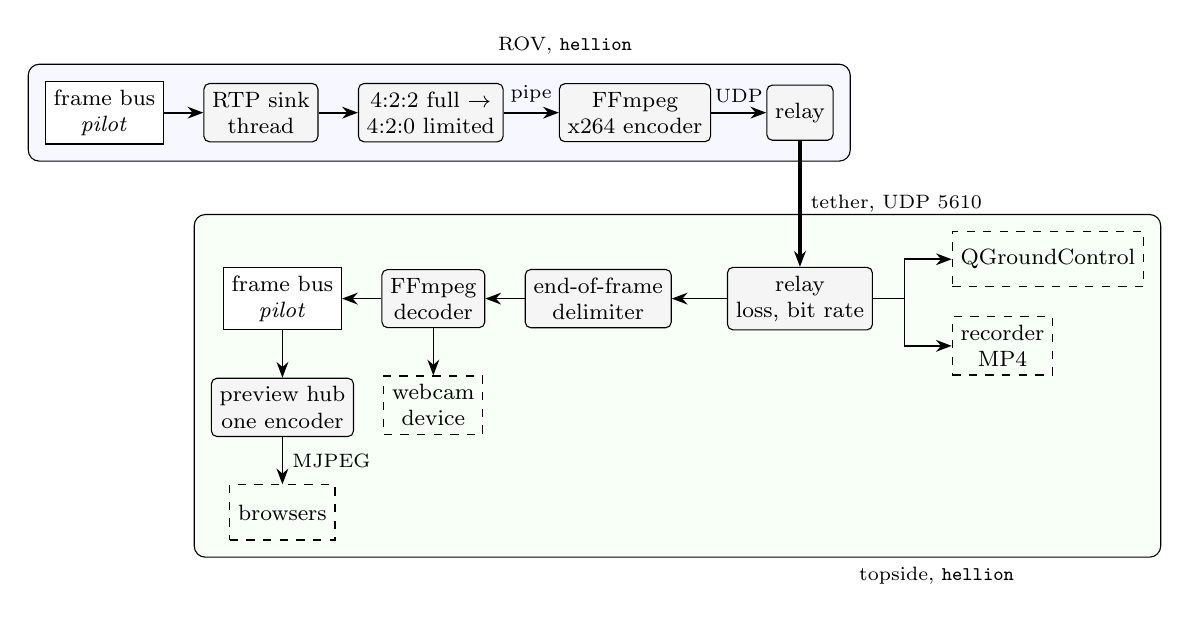
\begin{tikzpicture}[node distance=4mm and 5mm]
    \node[buf] (bus) {frame bus\\\emph{pilot}};
    \node[proc, right=of bus] (sink) {RTP sink\\thread};
    \node[proc, right=of sink] (conv) {4:2:2 full $\to$\\4:2:0 limited};
    \node[proc, right=7mm of conv] (enc) {FFmpeg\\x264 encoder};
    \node[proc, right=7mm of enc] (rel) {relay};
    \node[proc, below=16mm of rel] (trel) {relay\\loss, bit rate};
    \node[ext, right=10mm of trel, yshift=5mm] (qgc) {QGroundControl};
    \node[ext, right=10mm of trel, yshift=-6mm] (rec) {recorder\\MP4};
    \node[proc, left=7mm of trel] (aud) {end-of-frame\\delimiter};
    \node[proc, left=of aud] (dec) {FFmpeg\\decoder};
    \node[buf, left=of dec] (tbus) {frame bus\\\emph{pilot}};
    \node[proc, below=6mm of tbus] (hub) {preview hub\\one encoder};
    \node[ext, below=6mm of hub] (web) {browsers};
    \node[ext, below=6mm of dec] (v4l) {webcam\\device};
    \draw[flow] (bus) -- (sink);
    \draw[flow] (sink) -- (conv);
    \draw[flow] (conv) -- node[lab, above] {pipe} (enc);
    \draw[flow] (enc) -- node[lab, above] {UDP} (rel);
    \draw[net] (rel) -- node[lab, right] {tether, UDP 5610} (trel);
    \draw[flow] (trel.east) -- ++(4mm,0) |- (qgc.west);
    \draw[flow] (trel.east) -- ++(4mm,0) |- (rec.west);
    \draw[flow] (trel) -- (aud);
    \draw[flow] (aud) -- (dec);
    \draw[flow] (dec) -- (tbus);
    \draw[flow] (dec) -- (v4l);
    \draw[flow] (tbus) -- (hub);
    \draw[flow] (hub) -- node[lab, right] {MJPEG} (web);
    \begin{scope}[on background layer]
      \node[box, fill=blue!3, fit=(bus)(sink)(conv)(enc)(rel), label={[lab]above right:ROV, \hellion{}}] {};
      \node[box, fill=green!3, fit=(tbus)(dec)(aud)(trel)(qgc)(rec)(hub)(web)(v4l),
            label={[lab]below right:topside, \hellion{}}] {};
    \end{scope}
  \end{tikzpicture}
  \caption{Video transport in placement B. The vehicle's \hellion{} converts each frame
    to the encoder's format and relays the encoder's packets; topside, a relay owns the
    tether port, measures the link, and copies every packet to QGroundControl and the
    recorder unchanged and to the decoder followed by an end-of-frame delimiter. One
    preview encoder per stream serves all browsers.}\label{fig:transport}
\end{figure}

\begin{table}[pos=htbp]
  \centering\small
  \caption{Transport settings.}\label{tab:transport}
  \begin{tabular}{@{}L{3.3cm}L{10.2cm}@{}}
    \toprule
    Stage & Setting \\
    \midrule
    Encoder input & raw I420, limited range (Eq.~\ref{eq:range}), nominal frame rate \\
    Encoder & libx264 \citep{x264}, preset \texttt{ultrafast}, tune \texttt{zerolatency}
      (no B-frames, no look-ahead); 4\,000~kbit/s, maximum rate 4\,000~kbit/s,
      buffer 2\,000~kbit; keyframe every 30 frames; parameter sets before every keyframe \\
    Packetization & RTP, payload of at most 1\,200 bytes \\
    Tether & UDP port 5610 (QGroundControl's 5600 is left free) \\
    Decoder input & no input buffering, low-delay flags, no reordering wait;
      an access unit delimiter after each frame \\
    Decoder output & raw I422, full range, fixed size; slice threading \\
    Recording & stream copy into fragmented MP4, a fragment per keyframe \\
    Preview & MJPEG, 4:2:0, quality 75, $\approx$15 frames per second, one encoder per stream \\
    Restarts & encoder with back-off from 1 to 30~s; decoder at once, or after 5~s
      without output while packets arrive \\
    \bottomrule
  \end{tabular}
  \tablenote{The encoder can be replaced per pipeline, for example by a hardware encoder
    on the vehicle; the decoder side does not depend on the encoder.}
\end{table}

\subsection{Implementation and deployment}\label{sec:implementation}

Both programs are written in C99 and built by one GNU make file; they need a C99
compiler (GCC~4.7 or later, or Clang), libjpeg-turbo~1.4 or later and, for \hellion{},
FFmpeg at run time, and they run on Linux~3.2 or later. Release binaries are built
statically for x86-64, ARMv7 with NEON and AArch64 with GCC~15.3 (Bootlin toolchains
2026.08-1; \citealp{bootlin}) and libjpeg-turbo~3.2.0, so that they need no libraries
on the target. Child processes are started with their program resolved before
\texttt{fork}, with inherited file descriptors closed and signals reset, in their own
process group, and are stopped by closing their input before signalling them. An
installation script installs both programs as system services on each end of the
tether, given the end's role and the placement; the two services run as one service
user, so that \hellion{} can write \eeye{}'s configuration and both can use the frame
bus, and neither needs elevated privileges.

\subsection{Verification and measurement}\label{sec:verification}

The source carries 17 test suites, run on every build: the configuration parser, the
ring buffers, the JPEG decoding and framing, resolution negotiation, the operators and
the chain, the visibility correction, the camera controls, the raw recorder and the
webcam output, child processes, the frame bus under concurrent processes (including a
writer overtaking a reader during a copy), the health records, the HTTP server and
client, and \hellion{}'s pipelines, relay, status file and RTP round trip through
FFmpeg. The suites also run, as built for
release, on ARMv7 and AArch64 under QEMU user-mode emulation, which executes the NEON
paths. The HTTP parsers were fuzzed with libFuzzer, and the suites of the changed
components were run under AddressSanitizer and UndefinedBehaviorSanitizer.

Each change that should not alter the output was checked against the previous code by
hashing the output of both over a fixed set of inputs: three 1280$\times$720 camera
photographs and synthetic frames of edge-case sizes (odd chroma widths, frames one or
two pixels wide), every strength and threshold of the operator in steps, 1 to 7
threads, on x86-64 and on both ARM targets under emulation (Table~\ref{tab:equivalence}).
Processing costs were measured as the minimum over repeated runs on an AMD Ryzen~5
5600 (6 cores) with the threads of OpenMP set to sleep while idle, as \eeye{}
configures them; costs on ARM were estimated as executed instruction counts under QEMU
with an instruction-counting plugin, which reflects the work but not the memory
behaviour of a Raspberry Pi (Table~\ref{tab:costs}).

Transport latency was measured from frame bus to frame bus through two \hellion{}
processes, one as the vehicle and one as the topside, connected over loopback on an
idle laptop (AMD Ryzen~5 5600H, FFmpeg~9.0.2). A test program published frames whose
pixels encode their frame number and read them from the receiving bus; the latency of a
frame is the difference between the two times, and an RTP tap between the encoder and
the decoder divided it into stages (Table~\ref{tab:latency}). The complete chain was
also run between two machines on a local network, the laptop's built-in camera (HP
Wide Vision HD, UVC) serving as the vehicle's camera, for placements A and B, for the
camera controls in placement~A, for the recording and the decoder across disconnections
of the network cable, and for automatic pairing. Neither program has yet been run on the
vehicle.

\begin{table}[pos=htbp]
  \centering\small
  \caption{Transport latency, frame bus to frame bus through two \hellion{} processes
    over loopback; median (10th--90th percentile) of 300 frames.}\label{tab:latency}
  \begin{tabular}{@{}lccc@{}}
    \toprule
    & \makecell{640$\times$480\\30 frames/s} & \makecell{640$\times$480\\60 frames/s}
    & \makecell{1280$\times$720\\30 frames/s} \\
    \midrule
    Without the delimiter and slice threading & 70.4 (70.2--70.6)~ms & 37.0 (36.8--37.2)~ms & 74.8 (74.6--75.1)~ms \\
    With both & 3.8 (3.7--4.1)~ms & 3.7 (3.6--3.9)~ms & 8.3 (8.1--8.6)~ms \\
    \bottomrule
  \end{tabular}
  \tablenote{Without the two measures the decoder held two frame periods: about one in
    FFmpeg's H.264 parser and one in its raw video output. The encoder, from the frame
    written to its last RTP packet, took 1.2--1.5~ms at 640$\times$480, and \hellion{}'s
    own relay, pipe and bus about 0.5~ms. Camera exposure, the tether and the vehicle's
    encoder add to these figures.}
\end{table}

\begin{table}[pos=htbp]
  \centering\small
  \caption{Processing costs per 1280$\times$720 frame. x86-64: AMD Ryzen~5 5600,
    minimum over repeated runs, 4 threads unless stated. ARM: executed instructions under
    emulation, one thread, 20 frames.}\label{tab:costs}
  \setlength{\tabcolsep}{4pt}
  \begin{tabular}{@{}L{6.2cm}L{3.2cm}L{4.2cm}@{}}
    \toprule
    Stage & x86-64 & ARM (instructions) \\
    \midrule
    Image statistics and visibility correction & 0.55~ms (2.09~ms, 1 thread) & -- \\
    Blur, strength 1 & 0.18~ms & AArch64 183\,M; ARMv7 263\,M \\
    Blur, strength 4 & 0.59--0.66~ms & AArch64 283\,M; ARMv7 391\,M \\
    Blur, strength 8 & 0.84~ms & AArch64 486\,M; ARMv7 676\,M \\
    Blur, strength 20 & 1.56~ms & -- \\
    Canny, strength 2, thresholds 40/90 & 3.41--3.82~ms & -- \\
    Frame bus publication & 34.9~$\mu$s; 17.2~$\mu$s with neutral chroma & -- \\
    \addlinespace
    \hellion{} preview, 1 and 4 viewers & 4\% and 4\% of a core & -- \\
    Encoder (FFmpeg, libx264), 30 frames/s & 0.21~s of CPU per second of video, laptop & -- \\
    \bottomrule
  \end{tabular}
  \tablenote{Before the measures described in the text, the visibility correction took
    1.49~ms, the blur 0.75, 1.38 and 2.27~ms at strengths 1, 4 and 8 (and 900\,M and
    1\,108\,M instructions on AArch64 at 4 and 8), Canny 3.80--4.20~ms, the preview
    13\% of a core with four viewers, and the encoder 0.30~s of CPU per second of
    video.}
\end{table}

\begin{table}[pos=htbp]
  \centering\small
  \caption{Equivalence checks: output hashed over all cases for the previous and the
    revised code; every comparison was identical.}\label{tab:equivalence}
  \setlength{\tabcolsep}{4pt}
  \begin{tabular}{@{}L{3.6cm}L{6.2cm}rL{3.2cm}@{}}
    \toprule
    Change & Inputs & Cases & Platforms (threads) \\
    \midrule
    Visibility correction & smooth, flat and noisy synthetic sequences of 60 frames, at
      sizes from 1920$\times$1080 to 1$\times$1, including padded strides & -- & x86-64, AArch64, ARMv7 \\
    Canny & 3 photographs $\times$ 4 strengths $\times$ 7 low $\times$ 6 high thresholds & 504 & x86-64 (1, 3, 4), AArch64, ARMv7 (4) \\
    Blur, half-resolution NEON & 4 sizes $\times$ strengths 0--20 $\times$ 3 or 1 planes & 168 & x86-64 (1, 4), AArch64, ARMv7 (4) \\
    Blur, scratch-plane passes & 7 sizes, including 2-pixel-wide frames $\times$ strengths 0--20 $\times$ 3 or 1 planes & 294 & x86-64 (1, 3, 4), AArch64, ARMv7 (4) \\
    \bottomrule
  \end{tabular}
\end{table}

\section*{Code availability}

Name of the software: electric-eye (programs \eeye{} and \hellion{}). Developer:
H. O\u{g}uz Bolat, \href{mailto:oguz.bolat@std.yildiz.edu.tr}{\nolinkurl{oguz.bolat@std.yildiz.edu.tr}}.
Program language: C99. Hardware requirements: an x86-64, ARMv7 with NEON or AArch64 processor;
tested on desktop and laptop computers and, for the ARM builds, under emulation.
Software required: a C99 compiler, GNU make and libjpeg-turbo to build; FFmpeg at run
time for \hellion{}. The source code, its documentation and the release binaries are at
\url{https://github.com/hogib/electric-eye}; this description corresponds to release
v0.3.1 (commit 96b3eb1).

\section*{Declaration of generative AI and AI-assisted technologies in the manuscript preparation process}

During the preparation of this work the authors used Claude Opus~5.5 (Anthropic) to
develop parts of the software and to draft and edit the manuscript text. After using
this tool, the authors reviewed and edited the content as needed and take full
responsibility for the content of the published article.

\bibliographystyle{cas-model2-names}
\bibliography{refs}

\end{document}
